\documentclass[a4paper,14pt]{extarticle}
\usepackage[utf8]{inputenc}
\usepackage[T1]{fontenc}
\usepackage[french]{babel}
\usepackage{graphicx}
%Modification des marges de la feuille
\usepackage[left=3.0cm, right=2.3cm, top=3cm, bottom=2.5cm]{geometry}
\usepackage{hyperref}
%Permet d'accéder à la dernière page
\usepackage[table,xcdraw]{xcolor}
\usepackage{float}

% Permet de changer l'orientation de la page
\usepackage{pdflscape}

%afficher le code source
\usepackage{listings}
\usepackage{xcolor}

\usepackage{vhistory}

% Permet de changer la page de garde
\usepackage{fancyhdr, lastpage}

\newcommand{\DP}{David Paulino}

%Permet d'afficher le nombre de pages totale sur le document

\title{Football Prediction}
\author{\vhListAllAuthorsLongWithAbbrev}
\date{\today}

\makeatletter


\pagestyle{fancy}
%Entete + pied de page
\lhead{\DP}
\chead{\@title}
\rhead{\@date}
\lfoot{Version \vhCurrentVersion}
\cfoot{Page \textbf{{\thepage}} sur \textbf{\pageref{LastPage}}}
\rfoot{Rapport}

\begin{document}

%page de garde
  \begin{titlepage}
  \centering
      {\large \textsc{Centre de formation professionnelle technique}}\\
    \vspace{2cm}
    
    \vfill
       {\LARGE \textbf{\@title}} \\
    \vspace{1cm}
    \begin{figure}[H]
        \centering
        \includegraphics[width=7cm]{../img/logo_blackborder.png}
    \end{figure}
    \vspace{1cm}
        { \LARGE Manuel utilisateur}\\
    \vspace{2em}
        {\large \textbf{\@author}} \\
    \vspace{6em}
        {\large \@date}\\
    \vspace{1cm}
        {\large \textsc{Version \vhCurrentVersion}} \\
    \vfill
  \end{titlepage}
\makeatother

\newpage

\tableofcontents

{\setlength{\parindent}{0cm} % Remove indent on paragraph
\setlength{\parskip}{1em} % Add jump after paragraph

\newpage
%Versionning du document
\makeatletter

\begin{versionhistory}
    \vhEntry{1.0}{\today}{DP}{Version initiale}
\end{versionhistory}

\makeatother

\section{Introduction}

Ce document est destiné aux utilisateur de l'application web "Football Prediction". L'application a été réalisé dans le cadre du travail de diplôme de technicien pour l'obtention du diplôme de Technicien ES. Il s'agit d'une application qui permet de visualiser le résultat d'une prédiction sur un match entre 2 équipes de football. Cela permet à des pronostiqueurs de se baser sur ce travail pour avoir une source supplémentaire pour choisir leur mise lors d'un pari sportif.

Cette documentation est la pour montrer l'interface utilisateur et le détail des actions possibles par l'utilisateur.

\newpage

\section{Utilisation de l'application web}

\subsection{Menu de navigation}

\begin{figure}[htp]
    \centering
    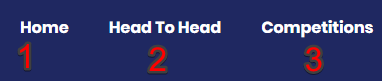
\includegraphics[width=20em]{./img/menu.png}
    \caption{Menu }
    \label{fig:menu}
\end{figure}

\begin{enumerate}
    \item Page d'accueil du site
    \item Page pour la fonctionnalité "Head To Head"
    \item Page pour la fonctionnalité "Competitions"
\end{enumerate}

\subsection{Page d'accueil}

\begin{figure}[H]
    \centering
    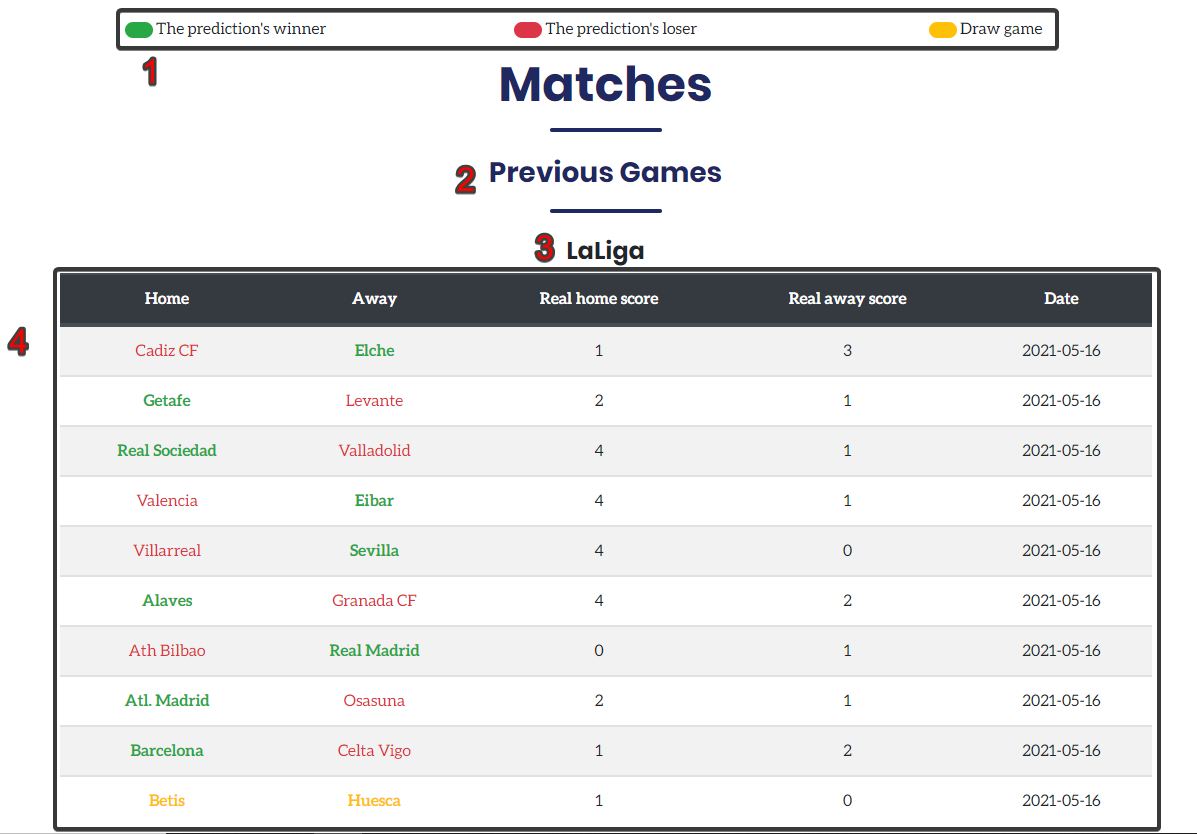
\includegraphics[width=30em]{./img/previousGamesHome.png}
    \caption{Page d'accueil - Matchs précédents}
    \label{fig:previousGamesHome}
\end{figure}

\begin{enumerate}
    \item Légendes pour expliquer le code couleur sur les matchs
    \item Les matchs précédents
    \item Nom de la ligue
    \item Liste des matchs pour la ligue
\end{enumerate}

Si on scrolle plus bas dans la page, la disposition est la même. On trouvera "Upcoming matches" et il manquera les "Real home score" et "Real away score" dans la liste des matchs.

\subsection{Page "Head To Head"}

Pour ouvrir les modales, il suffit de cliquer sur le bouton suivant (voir fig. \ref{fig:buttonOpenModal}). 

\begin{figure}[H]
    \centering
    
\includegraphics[width=3em]{./img/buttonOpenModal.png}
    \caption{Page Head To Head - Bouton ouverture modale}
    \label{fig:buttonOpenModal}
\end{figure}

\begin{figure}[H]
    \centering
    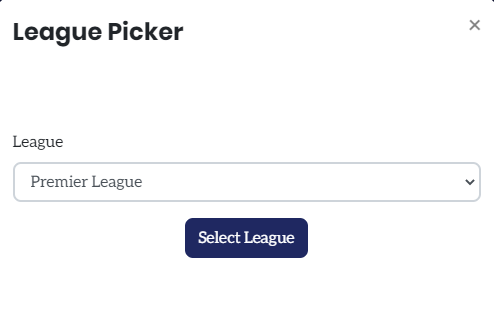
\includegraphics[width=25em]{./img/leagueSelection.png}
    \caption{Page Head To Head - Sélection de la ligue}
    \label{fig:leagueSelection}
\end{figure}

La modale ci-dessus permet de sélectionner la ligue.

\begin{figure}[H]
    \centering
    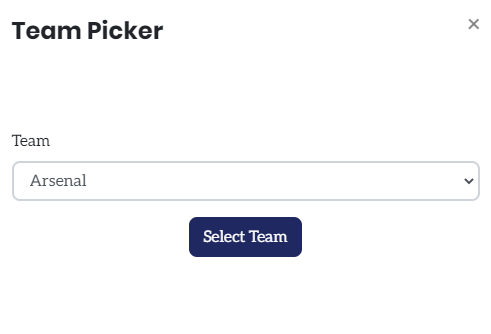
\includegraphics[width=25em]{./img/teamSelection.png}
    \caption{Page Head To Head - Sélection de l'équipe}
    \label{fig:teamSelection}
\end{figure}

Cette modale permet de sélectionner une équipe. Elle est la même pour la sélection des deux équipes.
Après avoir sélectionner une équipe, le blason de l'équipe en question s'affiche sur la page (voir fig. \ref{fig:teamsSelected}). 

\begin{figure}[H]
    \centering
    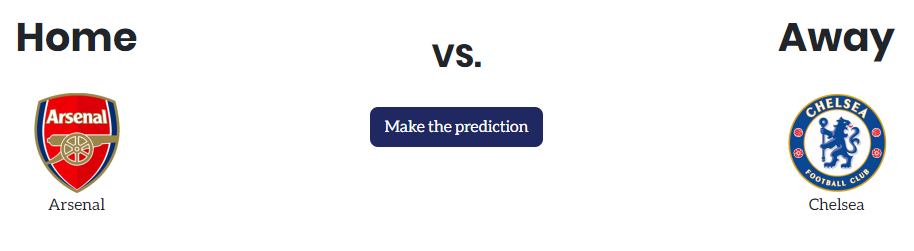
\includegraphics[width=30em]{./img/teamsSelected.png}
    \caption{Page Head To Head - Équipes sélectionnées}
    \label{fig:teamsSelected}
\end{figure}

Une fois les deux équipes sélectionnées, on a accès au bouton "Make the prediction". Après avoir cliqué dessus, un chargement apparaîtra à l'écran.

\begin{figure}[H]
    \centering
    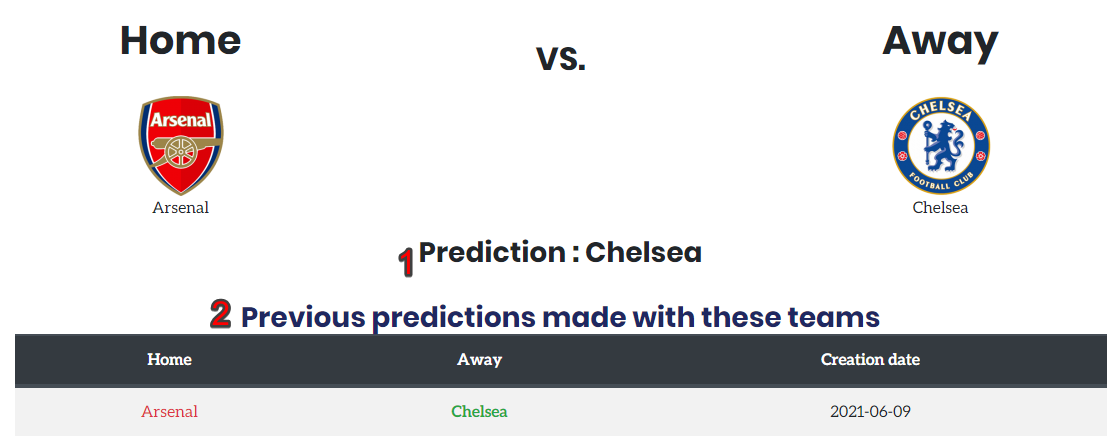
\includegraphics[width=30em]{./img/predictionMade.png}
    \caption{Page Head To Head - Prédiction faite}
    \label{fig:predictionMade}
\end{figure}

\begin{enumerate}
    \item Résultat de la prédiction
    \item Les prédictions précédentes faites entre les deux équipes
\end{enumerate}

\subsection{Page "Competitions"}

La sélection de la ligue est la même que pour la fonctionnalité "Head To Head" (voir figs. \ref{fig:buttonOpenModal} et \ref{fig:leagueSelection})

\begin{figure}[H]
    \centering
    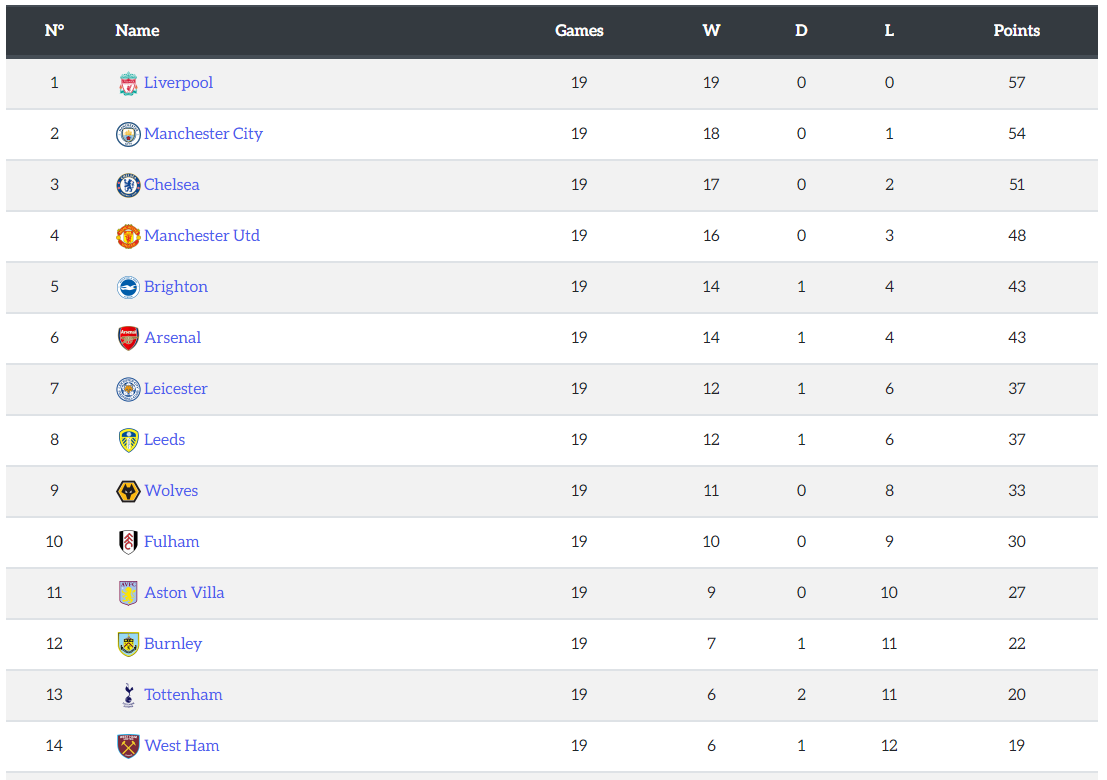
\includegraphics[width=27em]{./img/competitionStanding.png}
    \caption{Page Competitions - Prédiction sur la compétition faite}
    \label{fig:competitionPredictionMade}
\end{figure}

On voit bien le classement de la compétition, avec les points, les victoires, égalités et défaites. 

Note : C'est une prédiction sur une compétition toute entière.

On peut ensuite cliquer sur le nom de n'importe quelle équipe pour être rediriger vers l'historique des matchs de l'équipe en question dans la compétition.

\begin{figure}[H]
    \centering
    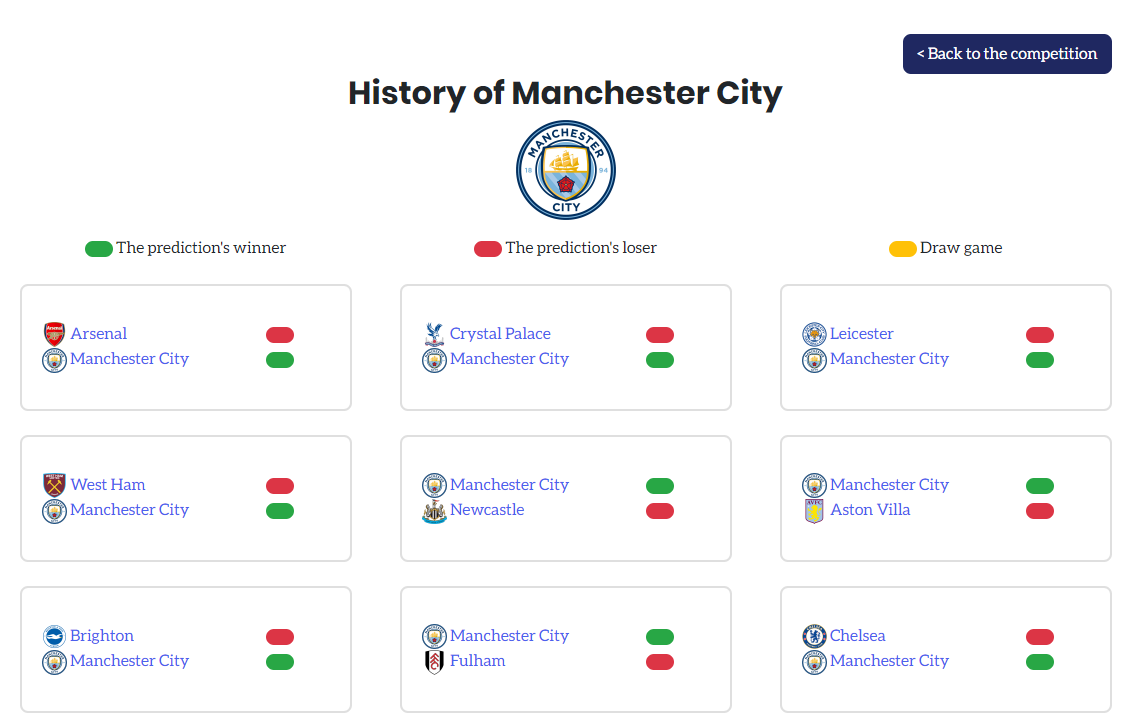
\includegraphics[width=27em]{./img/competitionHistory.png}
    \caption{Page Competitions - Historique des matchs d'une équipe dans la prédiction de la compétition}
    \label{fig:competitionHistory}
\end{figure}

On peut voir ici que l'on a l'historique des matchs avec l'expliquation des codes couleurs utilisés. On peut être directement dirigé vers l'historique d'une équipe depuis cette page en cliquant dessus.

\end{document}
